\chapter{基于DTW距离测度的Shapelet并行算法}
\label{cha:myalg}

第二章介绍了Shapelet的通用算法和基本定义,第三章介绍了GPU/CUDA并行原理、并行的难点,本章在前面介绍Shapelet和GPU/CUDA相关技术的基础上,提出了基于DTW距离测度的Shapelet并行算法。

本章首先~\ref{cha:myalg:Overview}介绍基于DTW距离测度的Shapelet并行算法总体流程、并行方案,整个流程主要定义~\ref{def:chap03:Threephases}的三个阶段:距离计算阶段(~\ref{cha:myalg:DTW},~\ref{cha:myalg:euclid})、最佳分割点计算阶段(~\ref{cha:myalg:infogain})、求最大信息增益阶段。

\section{算法总体流程}
\label{cha:myalg:Overview}

{\color{red}{如果更改几个框的名字,也需要改这一块,底下标题要改,Reduce求最小值也要改}}


\begin{figure}[H] % use float package if you want it here
	\centering
	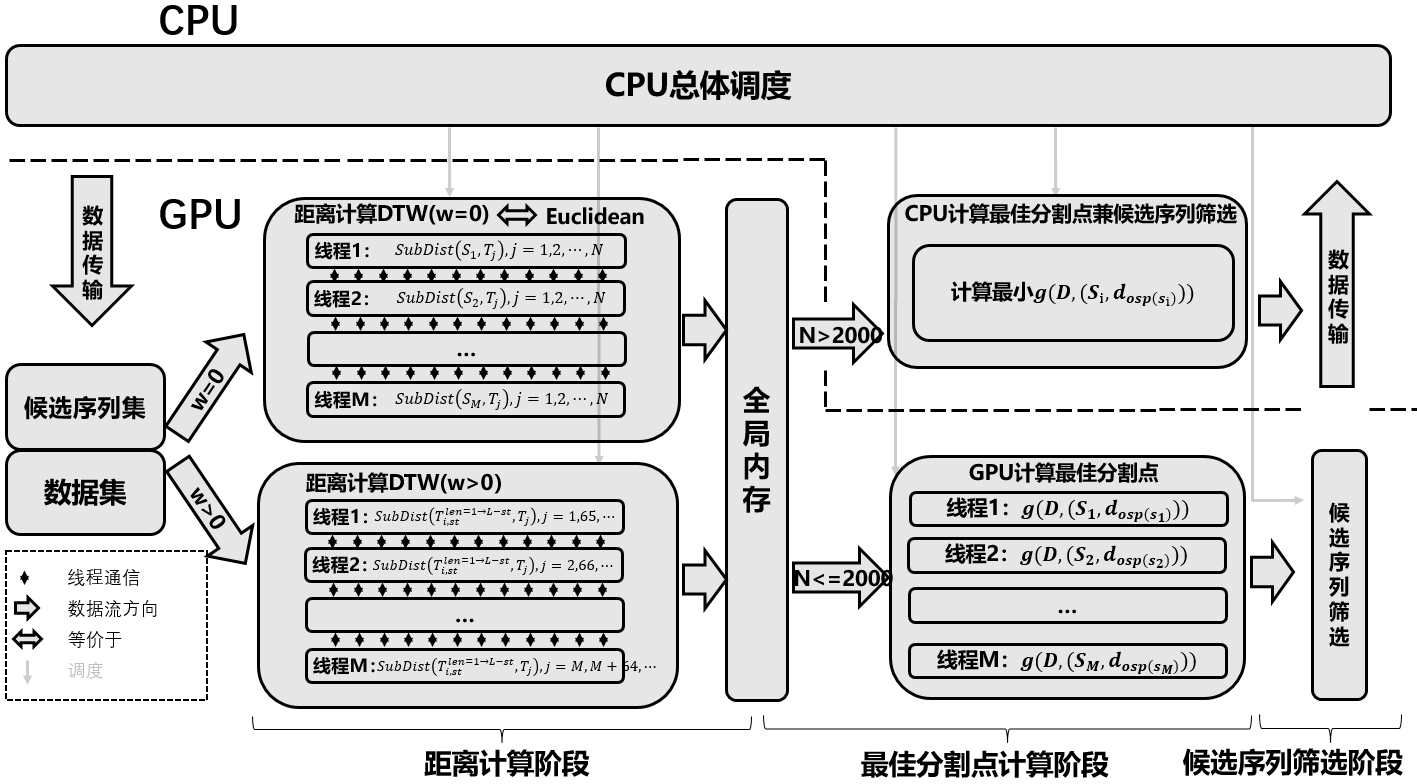
\includegraphics[height=8.2cm]{generalflowchart.png}
	\caption{Shapelet总体算法流程}
	\label{fig:generalflow}
\end{figure}
如图~\ref{fig:generalflow},DTW-Distance Shapelet算法分为三个阶段:

1.距离计算阶段:输入子序列$S$和数据集$D$,输出$\mathcal{F}$(见定义~\ref{def:chap2:SubDist},公式~\ref{equ:chap2:SubDistSet})。 

2.最佳分割点计算阶段:输入$\mathcal{F}$,输出信息增益$g(D,(S,d_{osp(S)}))$以及对应的$S$,$d_{osp(S)}$。

3.Reduce求最小值阶段:输入信息增益$g(D,(S,d_{osp(S)}))$以及对应的$S$,$d_{osp(S)}$,输出最小的信息增益以及其对应的$S$,$d_{osp(S)}$。
\subsection{测度距离选择}
{\color{red}{需要在这里叙述一下$w$变化的优点,也就是为什么采用$w$测度}} \\
因为大部分情况下,两个在整体具有相似形状的序列,它们在时间轴上并不是一一对齐的。
因为DTW可以覆盖欧式距离

\subsection{并行方案}
算法符合整体符合CPU调度,GPU执行数据计算部分的整体框架,但是数据计算部分会根据数据和参数的不同会有不同的分支处理。数据计算部分主要分为三个阶段:距离计算阶段、最佳分割点计算阶段、Reduction计算最大信息增益阶段。

距离计算阶段:在GPU中执行每个子序列$S$对于数据集每个时间序列,存储在全局内存中(global Memory)。当 ~$w>0$时,采用DTW测度,具体算法设计在章节~\ref{cha:myalg:DTW}。但当$w=0$时,DTW距离等价于欧氏距离,而且相比更加节省时间(见章节~\ref{chap02:euclid2Dtw}),具体设计在~\ref{cha:myalg:euclid}详细叙述。

最佳分割点(最大信息增益)计算阶段:这部分会根据数据集的大小( $N$)选择不同的分支。一般情况下,序列$S$对应最佳分割点的计算在GPU中执行。当$N$达到一定值时,GPU中运行时,每个Block要求有更多的寄存器和共享内存,但是硬件环境每个Block只能提供48K的共享内存和64K的寄存器大小(见表~\ref{tab:gpuversion}),因此这一部分放在CPU中执行。

Reduction计算最大信息增益阶段:在$O(NL^2)$(见定义~\ref{def:chap02:Subsequence})个子序列$S$对应的信息增益中求最大值。这一阶段的本质是一个长的数组求最小值,我们采用Parallel Reduction~\cite{harris2007optimizing}的算法,时间复杂度为$O(\log(N)+\log(L))$。因为这一部分相比前两部分时间时间占比不超过1\%,这里不做过多的详述。

CPU计算最佳分割点阶段( 计算最佳分割点的每个线程需要$O(N)$(数据集$D$中时间序列个数)空间,这些空间消耗的共享内存和寄存器,当$N$过大时,共享内存和寄存器使用超过GPU的内存限制,GPU将会上报资源不足,通过降低每个Block的线程个数也不能解决)采用的算法和GPU的最佳分割点计算是相同的,算法详见章节~\ref{cha:chap04::infogain}。运行过程是将多个候选序列$S$计算的结果$\mathcal{F}$从GPU拷贝的CPU,在GPU上逐个运行最佳分割点计算并取最小值。另外,使用CPU计算最佳分割点可以省略Reduce计算最大信息增益阶段。

全局内存:全局内存接受距离计算阶段的的结果$\mathcal{F}$,最佳分割点计算阶段再读取$\mathcal{F}$计算最大信息增益,相当于两个阶段之间的媒介。$\mathcal{F}$需要$O(N)$的空间复杂度,在全局内存中需要存储$O(NL^2)$个$\mathcal{F}$,因此,一次执行完所有流程使用全局内存空间复杂度至少为$O(N^2L^2)$。
数据集大小和时间序列长度增大都很容易导致全局内存不足。为了解决全局内存不足的问题,这里采用换入换出、分片计算的方法分多次执行,限制每次$\mathcal{F}$存储的最大数量(根据全局内存大小和$\mathcal{F}$(因数据集而不同)用内存大小计算)。

\section{距离计算并行算法设计}
\label{cha:myalg:DTW}
本章主要介绍$w>0$时,距离计算阶段并行所使用的并行策略、并行算法设计、以及并行技巧。在这一章讨论的都是基于$DTW(A,B,w)$距离讨论的。
\subsection{并行策略}


{\color{red}{在这里要注明每个线程要完成的事情,每个线程的空间复杂度,时间复杂度,均摊,复杂度这块也许可以放在算法设计阶段}}

在~\ref{cha:chap02:generalalganalysis}章节提及,距离计算$Dist(A,B)$时Shapelet算法中时间复杂度最高的操作,时间复杂度为$O(N^2L^4)$。但是部分距离之间存在着关系,可以通过这些距离之间的关系进行换算,避免每一个对距离计算都要花费$O(wL)$的时间。如图~\ref{fig:DTWParallel},在DTW测度距离$DTW(A_{1:M},B_{1:M},w)$过程中,涵盖了$M-1$个$DTW(A_{1:i},B_{1:i}),i=1,2,\cdots,M-1$距离结果,当每个$DTW(A_{1:i},B_{1:i}),i=1,2,\cdots,M$单独计算时,每个时间复杂度为$O(wM)$,总体时间复杂度为$O(wM^2)$;当$DTW(A_{1:i},B_{1:i}),i=1,2,\cdots,M$一起计算时,$DTW(A_{1:i+1},B_{1:i+1})$在$DTW(A_{1:i},B_{1:i})$的基础上计算,时间复杂度为$O(w)$,当使用这种增量的算法逐步计算所有DTW距离时,总的时间复杂度为$O(wM)$。

$SubDist(S,T_j)$是在$O(L)$个距离值中取最低值,根据上面提到的增量计算,$SubDist(S_{1:i+1},T_j)$在$SubDist(S_{1:i},T_j)$基础上计算的时间复杂度为$O(wL)$。$\mathcal{F}$包含$N$个$SubDist(S_{1:i+1},T_j)$计算,其中$j=1,2,\cdots,N$,则$\mathcal{F}_{S(1:i+1)}$在$\mathcal{F}_{S(1:i)}$基础上计算时间复杂度为$O(wNL)$。

在原始算法~\ref{alg:origin}中计算一个$\mathcal{F}$的时间复杂度为$O(NL^2)$,而$SubSet(D)$一共有$O(NL^2)$个子序列$S$,所以时间复杂度为$O(N^2L^4)$。在算法~\ref{alg:originplus}中,\textbf{第三行}$SubSetDiffStart(D)$只取$T_j,j=1,2,\cdots,N$中起始位置$st$不同的子序列$T_{j,st}^{L-st}$(该子序列的长度为$L-st$),因此$SubSetDiffStart(D)$集合大小为$O(NL)$。\textbf{第四、五行}是依次计算$\mathcal{F}_i,i=1,2,...$,\text{第五行}时间复杂度为$O(wNL)$,\textbf{第四行}循环进行$O(L)$。距离计算的时间复杂度为$O(wN^2L^3)$。

因为$SubDist(S,T_j)$中只需要计算出每个$DTW(S,T_{j,u}),u=1,2,\cdots,|S|$,并不需要知道$S$和$T_{j,u}$是如何对齐的。所以在计算$DTW(A,B,w)$并不需要$O(w|M|)$个空间,只需要能够满足$DTW(A_{1:i+1},B_{1:i+1})$在$DTW(A_{1:i},B_{1:i})$基础上计算即可,这样对于$DTW(A,B,w)$,空间复杂度为$O(2w)$。

{\color{red}{$SubDist(T_{i,s}^{1\to (L-s)}$,在文字部分体现一下每个线程都干了什么?}}


\begin{algorithm}
	\caption{Shapelet相关算法}
	\label{alg:originplus}
	\begin{algorithmic}[1]
		\Function{ShapeletAlg}{$D$}
		%\State $CENTER \gets (w+1)/2$;
			\State $lastS \gets \phi, lastinfogain \gets 0, lastdosp \gets 0$
			\ForAll{$S \in SubSetDiffStart(D)$}
				%\State $\mathcal{F} = \left\lbrace (...,SubDist(S,T_j),y_j),...\right\rbrace,j = 1,2,\cdots,N$
				\For{$i = 1$ to $|S|$}
					\State 在$\mathcal{F}_{S(1:i-1)}$的基础上计算$\mathcal{F}_{S(1:i)}$($i=1$直接计算)
					\State 计算$g(D,(S,d_{osp(S(1:i))}))$
					\If{$g(D,(S,d_{osp(S)})) > lastinfogain$}
						\State $lastinfogain \gets g(D,(S,d_{osp(S)}))$,$lastS\gets S$,$lastdosp\gets d_{osp(S)}$
					\EndIf
				\EndFor
			\EndFor
			\State \Return $lastinfogain,lastS,lastdops$
		\EndFunction
	\end{algorithmic}
\end{algorithm}

\begin{figure}[H] % use float package if you want it here
	\centering
	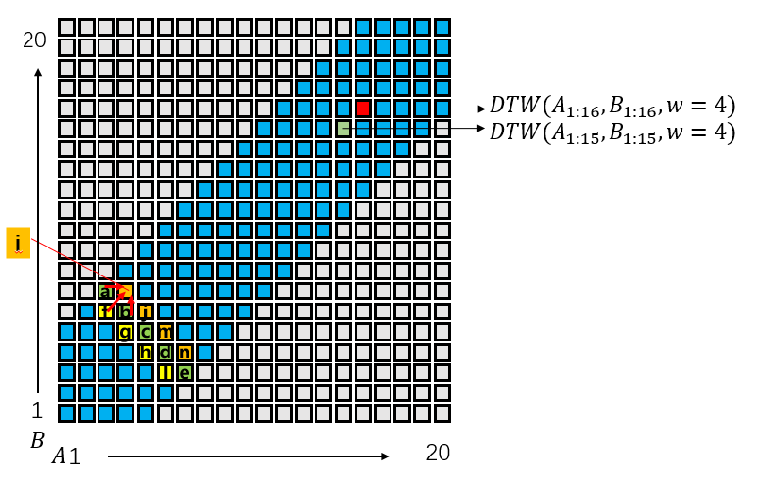
\includegraphics[height=8.2cm]{DTWParallel.png}
	\caption{DTW并行}
	\label{fig:DTWParallel}
\end{figure}

\subsection{并行算法设计}

如图~\ref{fig:DTWglobalMem},每个线程需要完成一个或者几个$SubDist(S,T_j)$计算,时间复杂度为$O(wL^2)$。

可以在这里加一个并行图。

\begin{figure}[H] % use float package if you want it here
	\centering
	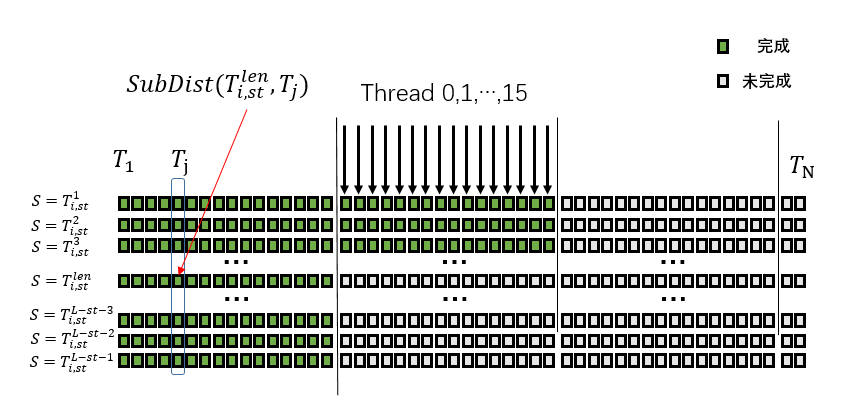
\includegraphics[height=8.2cm]{DTWglobalMem.png}
	\caption{执行顺序}
	\label{fig:DTWglobalMem}
\end{figure}

一共$O(N^2L)$个线程.
\begin{algorithm}
	\caption{$Block(i,s)$中$j$线程计算$SubDist(T_{i,s}^{1\to (L-s)},T_j)$}
	\label{alg:kernel_ComputedtwsperblockForAll}
	\begin{algorithmic}[1]
		%\Require ~~\\
		%$T_{i,s}^{1 \to (L-s)}$: $T_i$中以$s$为起始的$L-s$个子序列\\
		%$(idx,len)$:GPU计算中的一个block,满足$idx < N,len < L$;\\
		%$T_j$:整个事件序列;\\
		%\Ensure ~~\\
		%$dist$:$T_{idx,s}^{len}$相对于每个时间序列的距离组成的数组
		\Function{kernel\_Computedtwsperblock}{$T_{i,s}^{1 \to (L-s)},T_j,w$}
		%\State $CENTER \gets (w+1)/2$;
			\ForAll{$j \in thread_x$}
				%SubDist过程,比较L-s+1次
				\For{$u$ = $0$ to $L$}
					\State $odd \gets \left\lbrace \infty\right\rbrace$,$even \gets \left\lbrace \infty\right\rbrace$,$even[center] \gets 0$
					\For{$step$ = $1$ to $longest$}
						%\State Calc the location of the most left-up point:$x_0,y_0$
						\State 计算反对角线左上起点坐标$x_0,y_0$
						\For{$i$ = $tid$ to $2*w+2$}
							\State $x \gets x_0 + i, y \gets y_0 - i$
							\If{$x,y \in prunedtw$}
								\State $even[i] = (T_{j,x}-T_{idx,y})^2 + \min(even[i],min(odd[i],odd[i+1]))$
							\EndIf
						\EndFor
						%这里需要定义一个Dist(T_i^len,T_j);
						\State Compare the $even[center]$($Dist(T_{idx,st}^{step},T_{j,u})$) with prior $Dist(T_{idx,st}^{step},T_j)$ and save the minimum.
						\State Calc the location of the most left-up point:$x_0,y_0$
						\For{$i$ = $tid$ to $2*w+2$}
							\State $x \gets x_0 + i, y \gets y_0 - i$
							\If{$x,y \in prunedtw$}
								\State $odd[i+OFFSET_{odd}] = (T_{j,x}-T_{idx,y})^2 + \min(odd[i++OFFSET_{odd}],min(even[i],even[i+1]))$
							\EndIf
						\EndFor
					\EndFor
				\EndFor
			\EndFor
		\EndFunction
	\end{algorithmic}
\end{algorithm}

\subsection{实现细节与性能考虑(GPU)}

前两部分介绍了Shapelet并行策略和算法,这一部分就一些实现细节进行了阐述。

初始化有一个$\infty$赋值过程.
Coalesced
算法的极限。
共享内存使用。

线程Bankconfict,这个算法有的可能性比较大。

Block参数的讨论.需要确定出最佳的参数

1.DTW并行图放在这个里面,对应那几行代码?
2.Coalesced在这里的使用,哪几行使用了Coalesced
global Mem设计;label
3.在Share Mem允许下变化blocksize参数

{\color{red}{Trick部分还可以体现一下DTW的多线程运行}}

\section{$w=0$距离计算并行算法设计}
\label{cha:myalg:euclid}

当$w=0$时,DTW距离等价于欧氏距离,但是DTW距离相比欧氏距离多$O(L)$个比较操作和访存操作($L$为时间序列长度)。本章主要介绍$w=0$距离计算阶段的并行策略、并行算法设计以及实现细节和性能考虑。

\subsection{并行策略}

当候选序列$S=T_{i,s}^len$,每个线程需要进行$SubDist(S,T_j),j=1,2,\cdots,N-len$

这里画图距离$SubDist(T_{i,s}^{len},T_j),s=1,2,\cdots,N-len$

最基本元素是$Euclid(T_{i,s}^{len},T_{j,p}^{len})$

这里面也使用了重用策略,

{\color{red}{看看前面有没有关于$T_{i,j}$和$T_{i,j}^{len}$的定义}}

\begin{equation}
\label{equ:chap04:eucliddef}
Dist(T_{i,s}^{len},T_{j,p}^{len}) = \sum_{m=0}^{len-1}d(T_{i,s+m},T_{j,p+m})
\end{equation}

如果要使用下面递推式,就必须先有两个侧边的计算。

\begin{equation}
\label{equ:chap04:euclid}
Dist(T_{i,s+1}^{len},T_{j,p+1}^{len}) = Dist(T_{i,s}^{len},T_{j,p}^{len}) + d(T_{i,s+len},T_{j,p+len}) - d(T_{i,s},T_{j,p})
\end{equation}
{\color{red}{上面图指一下位置,侧边计算}}

{\color{red}{这个算法每个线程都是均匀的}}

\begin{figure}[H] % use float package if you want it here
	\centering
	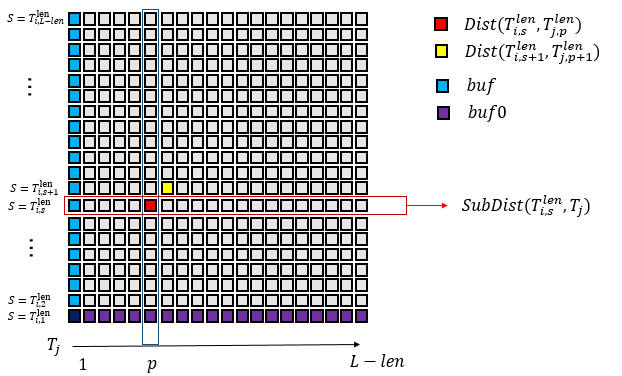
\includegraphics[height=8.2cm]{euclidparallel.png}
	\caption{$T_i$下长度为$len$的候选序列对于$T_j$的距离计算($w=0$)}
	\label{fig:euclidparallel}
\end{figure}


这里只能叙述一下线程中的一个循环的loop

这里需要包括并行策略和算法
\subsection{并行算法设计}

{\color{red}{在前面是否需要定义一个关于$SubDist(T_{i,s}^{len},D)$, 关于$T,D,T_i$等的关系,函数名也要也要统一}}

{\color{red}{而且这里面的算法都是存入GPU,而不是返回的,有可能要去掉返回值}}

单线程时间复杂度.

\begin{algorithm}
	\caption{计算$dist(T_{i,s}^{len},D)$,线程s,块(idx,len)}
	\label{alg:kernel_ComputeDist}
	\begin{algorithmic}[1]
		\Require ~~\\
		$T_{idx,s}^len$:$block(idx,len)$下线程$s$对应的{\color{red}{候选序列}}\\
		$(idx,len)$:GPU计算中的一个block,满足$idx < N,len < L$\\
		$T$:整个事件序列
		\Ensure ~~\\
		$dist$:$T_{idx,s}^{len}$相对于每个时间序列的距离组成的数组
		%\Function{kernel\_ComputeDist}{$T_{i}$}
		\For{$j$ = $1$ to $N$}
			\State $buf0[s]$ $\Leftarrow$ $0$;
			\State  $buf[s]$ $\Leftarrow$ $0$;
			\For{$i$ = $1$ to $len$} 
				\State $buf0[s]$ $\Leftarrow$ $buf0[s]$ + $(T_{idx,i}-T_{j,s+i})^2$;  \label{cccccc}
				\State $buf[s]$ $\Leftarrow$ $buf[s]$ + $(T_{idx,i+s}-T_{j,s})^2$;
			\EndFor
			\State $dist[j] = buf[s]$;
			%\State $syncthreads()$;
			\For{$u$ = $1$ to $L-len+1$}
				%\State $syncthreads()$;
				\If{$0 \neq s$}  
					\State $buf[s]$ $\Leftarrow$ $buf[s-1]$ + $(T_{idx,s+len}-T_{j,u+len})^2$ - $(T_{idx,s}-T_{j,u})^2$;
				\EndIf
				%\STATE $syncthreads()$;
				\If{$s$ is $0$}
					\State $buf[s]$ = $buf0[u]$;
				\EndIf
				\State $dist[j]$ $\Leftarrow$ $min(dist[j],buf[s])$
			\EndFor
		\EndFor
		\Return $dist$
	\end{algorithmic}
\end{algorithm}

\subsection{实现细节与性能考虑}

下面代码可以边实验边写

上面代码存在Warp divergence,序列化,而且有可能产生歧义。

关于dist的设计,这里使用了Coalseced的

line~\ref{cccccc},这段代码一定要并行计算,否则会成为时间瓶颈。

{\color{red}{可能不需要下面这段思路了,直接使用下下段就可以了}}
存储进入GM的方式.每16个元素存储一次,首先一个线程最多1024个线程.将连续写个占有很小空间,有可能当是的速度慢就出在这里了.这里很可能要用一个 Bank-Conflict.

多个S计算的距离同时存入,这个要把性能记下来,这里就需要一个transpose过程,和128要不要结合计算.

\section{启发式算法计算最佳分割点}
\label{cha:myalg:infogain}

{\color{red}{到底求最大信息增益还是求最小条件熵,这个可以在后面解释一下}}

最佳分割点计算阶段是根据距离计算阶段的结果$\mathcal{F}$,求出一个分割点$d_{osp(S)}$使得分割点两边的信息增益$g(D,(S,d_{osp(S)}))$最大。

算法~\ref{alg:OriginInfogain}为计算最大信息增益的算法,其中Line~\ref{code:sort}是对于$mathcal{F}$排序,时间复杂度为$O(N\log(N))$,Line~\ref{code:maxinfogain}为以步进的方式计算最大信息增益以及最大信息增益对应的分割点,时间复杂度为$O(N)$。因此对于单个子序列$S$相对$mathcal{F}$计算最大信息增益的时间复杂度为$O(N\log(N))$,但是对于整个子序列集合$SubSet(D)$,时间复杂度度为$O(N^2L^2\log(N))$。

{\color{red}{这个函数应该重写一些,名字统一,起什么名字,查一下论文}}

\begin{algorithm}
	\caption{$SplitInfogain$}
	\label{alg:OriginInfogain}
	\begin{algorithmic}[1]
%		\Require $dist$数组,$label$数组
%		\Ensure $infogain$,$dividepoint$,$leftis$
		\Function {Infogain}{$dist, label, N$}
			\State Sort $\mathcal{F}$ by first element \label{code:sort}
			\State 计算最大信息增益/最佳分割点 \label{code:maxinfogain}
%			\For{$i=0$ to $N-1$} \label{code:}
%				\State 计算$g(D,(S,d_{th}))$
%			\EndFor
		\EndFunction
	\end{algorithmic}
\end{algorithm}

{\color{red}{这一块关于原始算法再说点,尽量说为什么时间很长.将这个说成时间复杂度可以和最高时间复杂度可以比拟的环节}}

\subsection{启发式算法设计}

{\color{red}{这一部分需要怎么叙述会更清晰一些}}


最佳分割点计算的目的在于寻找一个距离阈值$d_{osp(S)}$使得获得的信息增益$g(D,(S,d_{osp(S)}))$尽可能大。根据公式~\ref{equ:chap2:Infogain2},可得信息增益最大化等价于条件熵$H(D|(S,d_{th}))$最小化\footnote{条件熵$H(D|(S,d_{th}))$恒大于$0$}。

图~\ref{fig:distancedistribute}为子序列$S$相对于数据集$D$的(距离,类标)集$\mathcal{F}$,横轴表示时间序列在数据集中的位置,纵轴表示$S$与时间序列$T_i$之间的距离$SubDist(S,T_i)$,颜色表示$T_i$的类标(A/B)。
\begin{figure}[H] % use float package if you want it here
	\centering
	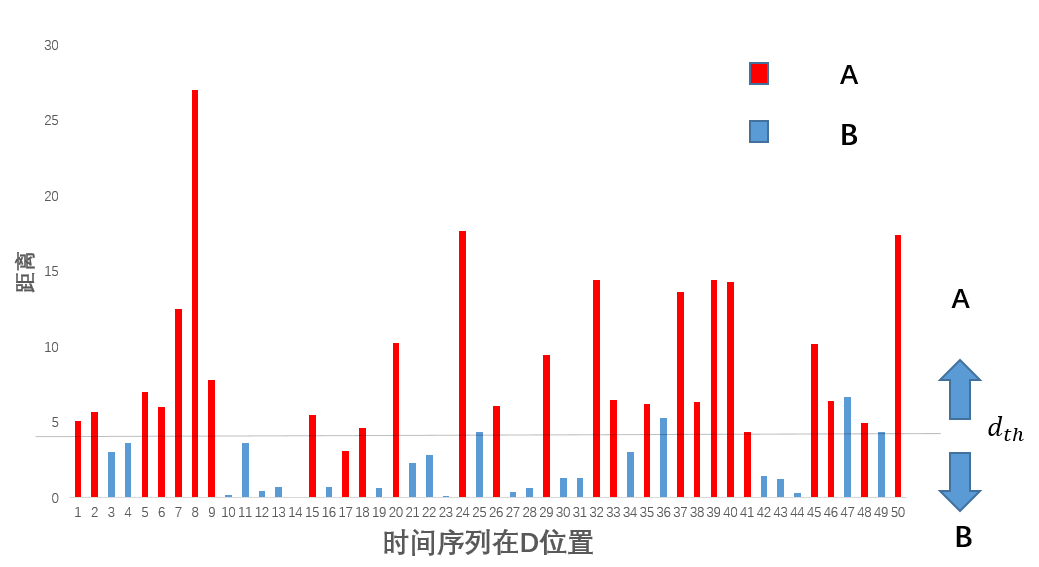
\includegraphics[height=5.2cm]{distancedistribute.png}
	\caption{$S$对于数据集$D$中时间序列的距离及类标,$\mathcal{F}$}
	\label{fig:distancedistribute}
\end{figure}

已知存在一个点$d_{th}$将数据集$D$分为两个子集$D_1 = \left\lbrace T,SubDist(S,T)<d_{th} \& T\in D\right\rbrace $和$D_2 = \left\lbrace T,SubDist(S,T) \geq d_{th}\& T\in D\right\rbrace$。对于数据集$D$来说,$|D|$为常数,可以将$\frac{|D_m|}{|D|}H(D_m),m=1,2$定义为$f(D_m),m=1,2$。
\begin{equation}
\label{equ:chap4:ConditionalEntropy}
H(D|(S,d_{th})) = \frac{|D_1|}{|D|}H(D_1)+\frac{|D_2|}{|D|}H(D_2) = f(D_1) + f(D_2)
\end{equation}

我们的目的是最小化$H(D|(S,d_{th}))$,为了使$H(D|(S,d_{th}))$变得更小,$f(D_m)$大的方向会有可能有一个点$d_{th2}$,使得$H(D|(S,d_{th2}))$更小。
刚开始在$(0,\infty)$之间搜索,之后再$(d_{th},\infty)$之间搜索,
参考快排的做法,取$\mathcal{F}$最后一个距离点作为分割点$d_{th}=\mathcal{F}_{N,1}$,如果$f(D_1)>F(D_2)$,则需要在寻找一个小于$d_{th}$的方向继续搜索最佳分割点,反之则在大于$d_{th}$的方向搜索
我们最终需要找到一个分割点$d_{osp(S)}$,使得条件熵$H(D|(S,d_{th}))$最大,
这是一个真实$S$相对$D$的距离$\mathcal{F}$,其中高度表示距离,颜色表示类标,
这里我们可以使用启发式的算法来计算最佳分割点,  

{\color{red}{提及一下最佳分割点的搜索方式}}

\begin{algorithm}
	\caption{使用启发式算法计算最佳分割点}
	\label{alg:HeuristicSplitInfogain3}
	\begin{algorithmic}[1]
		\Function {HeuristicSplitInfogain}{$dist,label,N,suma,sumb$}
			\State $left \gets 1,right \gets N$
			\While{$left < right$}
				\State $p \gets $ \Call{Partion}{$dist, label, left, right$}
				%\State $lefta2 \gets $ \Call{Count\_if}{$label,left,p,0$}
				\State $lefta \gets \sum_{i\in BEFORE(p)}(label_i\in A)$ \label{afterpartion}
				\State $leftb \gets \sum_{i\in BEFORE(p)}(label_i\in B)$
				\State $righta \gets  \sum_{i \in BEHIND(p)}(label_i \in A)$
				\State $rightb \gets  \sum_{i \in BEHIND(p)}(label_i \in B)$
				%\State $pgoleftentropy \gets$
				\State $leftentropy \gets $ \Call{Entropy}{$lefta,leftb$}
				\State $leftentropy \gets $ \Call{Entropy}{$righta,rightb$} \label{afterpartion2}
				\If{$leftentropy < rightentropy$}
				%\State $lefta1,leftb2 \gets lefta1 + lefta2,leftb1+leftb2$
				%\State 
					\State $left \gets p+1$
				\Else
				%\State $righta1,righta2 \gets righta1 + righta2,rightb1+rightb2$
					\State $right \gets p-1$
				\EndIf
				\If{$lastEntropy$ < $thisEntropy$}
					\State \Return $lastEntropy$
				\EndIf
			\EndWhile
			\State \Return $thisEntropy$
		\EndFunction
	\end{algorithmic}
\end{algorithm}


\subsection{shffule及其作用}

章节~\ref{cha:chap02:def}提及Shapelet的定义和本质,存在一种模式,数据中一种时间序列和这种模式表现出较小的距离,另外一种则表现出较大的距离,Shapelet的本质是寻找这种模式。与这种模式表现出较小距离的时间序列都存在能够表达这种模式的子序列,表明能够表达这种模式的子序列不止一个。

{\color{red}{”是否需要解释一下局部集合和分类模式",$SubDist(S1,T),SubDist(S2,T)$看一下这两段叙述的距离是否合理}}


能够表达这种特定模式的子序列对于数据集中各时间序列表现出相似的距离测度。如图~\ref{fig:similardistance},$S1$、$S2$是两个能够区分两种时间序列的子序列,两者相对于数据中各时间序列的距离很接近。如果使用上述启发式算法,最佳分割点的搜索路线有可能是一致的,因为上述算法都是使用局部集合的最后一个元素对于整个集合进行切割。

\begin{figure}[H] % use float package if you want it here
	\centering
	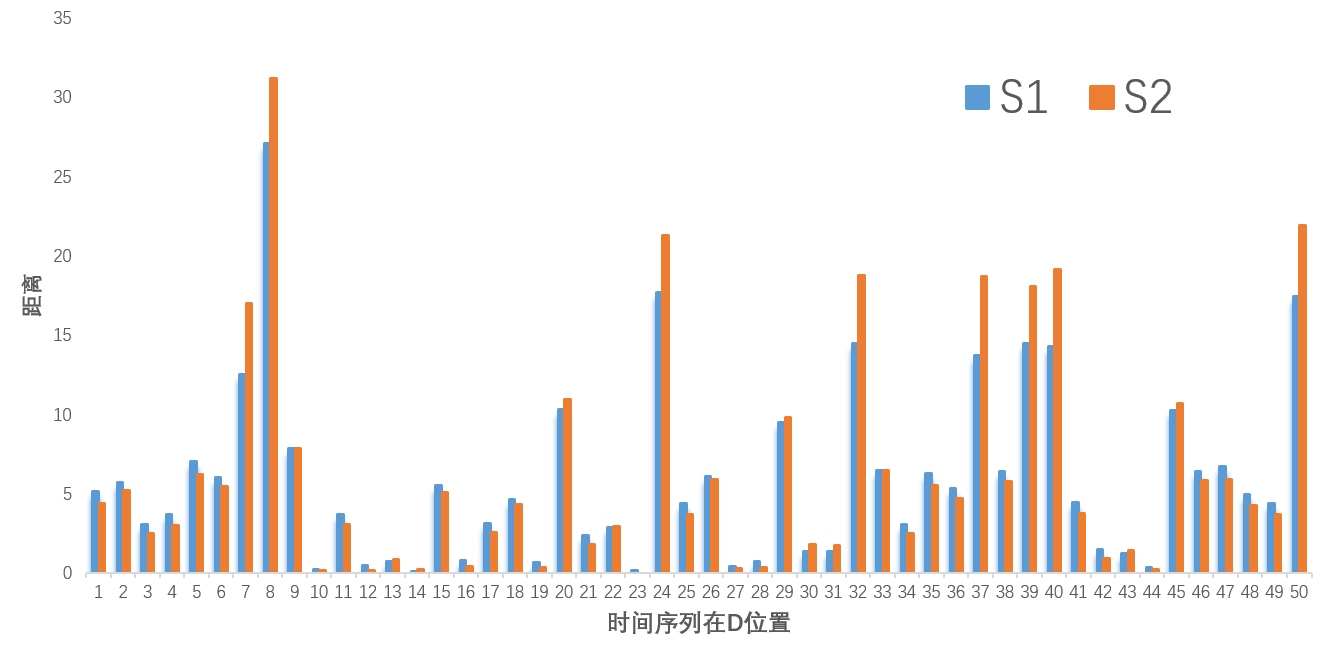
\includegraphics[height=8cm]{similardistance.png}
	\caption{$S1,S2$对于数据集$D$中时间序列距离的相似性}
	\label{fig:similardistance}
\end{figure}

启发式算法寻找的不是全局最优值,并不能保证这种唯一的搜索路线就能找最佳分割点。我们需要利用多个子序列能够表达这种模式这一特性,使多个子序列对应的启发式算法尽可能选择不同的最佳分割点搜索方式,目的是其中某种搜索方法式获得的结果和全局最优最接近。

为了获得不同的最佳分割点搜索方式,再进行启发式算法搜索之前,对于$\mathcal{F}$进行随机排列Shuffle。算法~\ref{alg:ReservoirShuffle}是随机排列算法伪码,本文选择蓄水池抽样算法进行随机排列,算法选择原因在章节~\ref{cha:chap04:Heuristic:Skill}中介绍。

\begin{algorithm}
	\caption{对于$dist$和对应的$label$进行shuffle,$ReservoirShuffle()$}
	\label{alg:ReservoirShuffle}
	\begin{algorithmic}[1]
		\Require ~~\\
		$dist$:一个{\color{red}{候选序列}}$S$对数据集$D$时间序列的距离数组\\
		$label$:对应label\\
		$seed$:某个线程的随机种子
		\Ensure ~~\\
		$dist$:shuffle之后的$dist$\\
		$label$:shuffle之后的$label$
		\Function {ReservoirShuffle}{$dist, label, N$}
			\For{$i$ = $2$ to $N$}
				\State $j$ $\gets$ \Call{random}{$1,i$}
				\If{$i \neq j$}
					\State \Call{swap}{$dist,i,j$}
					\State \Call{swap}{$label,i,j$}
				\EndIf
			\EndFor
			\State \Return $dist$,$label$
		\EndFunction
	\end{algorithmic}
\end{algorithm}

%伪码6
\begin{algorithm}
	\caption{使用启发式的方法计算最大熵以及最优分割点$HeuristicSplitInfogain${\color{red}{这个伪代码检查一下0和1,可能需要重新设计}}}
	\label{alg:HeuristicSplitInfogain}
	\begin{algorithmic}[1]
	\Require $dist$数组,$label$数组
	\Ensure $infogain$,$dividepoint$,$leftis$
	\Function {partion}{$dist, label, left, right$}
		\State $pivot$ $\gets$ $dist[right]$
		\State $p$ $\gets$ $left$
		\For{$q$ = $left$ to $right$}
			\If{$dist[q] < pivot$}
				\State \Call{swap}{$dist,p,q$}
				\State \Call{swap}{$label,p,q$}
				\State $p$ ++
			\EndIf
		\EndFor
		\State \Call{swap}{$dist,p,right$}
		\State \Return $p$
	\EndFunction
	
	\Function{Entropy}{$a,b$}
		\If{$a$ \textbf{is} $0$ \textbf{or} $b$ \textbf{is} $0$}
			\Return $0$
		\EndIf
		\State $pa \gets a/(a+b)$
		\State $pb \gets b/(a+b)$
		\State \Return $-(pa*\log(pa)+pb*\log(pb)$
	\EndFunction
	
	\Function{EntropySplit}{$lefta,leftb,righta,rithgb$}
		\State \Return $((lefta + leftb)*$\Call{Entropy}{$lefta,leftb$} $+(righta+rightb)*$ \Call{Entropy}{$righta,rightb$} $)/(lefta+leftb+righta+rightb)$;
 	\EndFunction
	\end{algorithmic}
\end{algorithm}

\subsection{实现细节与性能考虑(GPU)}
\label{cha:chap04:Heuristic:Skill}

这里对于随机排列算法进行一次评价,是否调用现成算法

对于启发式算法之前的随机排列,本算法通过蓄水池抽样算法完成,
使用share memory + coalseced 从GM copy出来.

理论计算Warp个数?

不可能使用生成一个随机序列,然后根据index进行shuffle,不要忘了算法随机种子的事。


\section{本章小结}






